\documentclass[12pt,twoside]{article}
\usepackage{light}
\usepackage{subfigure}
\usepackage{graphicx}
%\hidesolutions
\showsolutions


\begin{document}



\begin{problem}{15} 

\bparts

\ppart{5}

    For the graph in Figure~\ref{scc-graph}, compute the first two iterations
    of PageRank, starting from uniform PageRank values across all vertices.

    \begin{figure}[h!]
    \begin{center}
        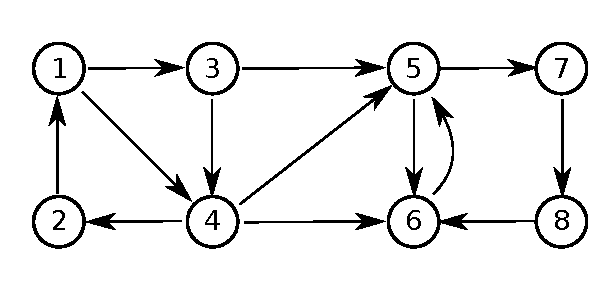
\includegraphics{ps6-scc-graph.pdf}
        \caption{A graph of web pages and links.}
        \label{scc-graph}
    \end{center}
    \end{figure}

    \solution{
        In the table below, we write the PageRank value of each vertex at
        iterations $0$, $1$, and $2$. We also include, for each vertex, the
        individual contributions made to that vertex in computing the next
        stage, which are summed in computing the following PageRank value.

        \begin{center}
        \begin{tabular}{r|cccccccc}
            & 1 & 2 & 3 & 4 & 5 & 6 & 7 & 8 \\
            \hline \\[-0.5em]
            iter 0  & $\frac18$ & $\frac18$ & $\frac18$ & $\frac18$ & $\frac18$ & $\frac18$ & $\frac18$ & $\frac18$ \\[1em]
            contrib & $\frac18$ & $\frac1{24}$ & $\frac1{16}$ & $\frac1{16}, \frac18$ & $\frac18, \frac1{16}, \frac1{24}$ & $\frac18, \frac1{16}, \frac1{24}$ & $\frac1{16}$ & $\frac18$ \\[1em]
            iter 1  & $\frac18$ & $\frac1{24}$ & $\frac1{16}$ & $\frac18$ & $\frac{11}{48}$ & $\frac{11}{48}$ & $\frac1{16}$ & $\frac18$ \\[1em]
            contrib & $\frac1{24}$ & $\frac1{24}$ & $\frac1{16}$ & $\frac1{16}, \frac1{32}$ & $\frac1{24}, \frac1{32}, \frac{11}{48}$ & $\frac18, \frac1{24}, \frac{11}{96}$ & $\frac{11}{96}$ & $\frac1{16}$ \\[1em]
            iter 2  & $\frac1{24}$ & $\frac1{24}$ & $\frac1{16}$ & $\frac3{32}$ & $\frac{29}{96}$ & $\frac{9}{32}$ & $\frac{11}{96}$ & $\frac1{16}$ 
        \end{tabular}
        \end{center}
    }

\ppart{10}

    Suppose that a graph $G$ consists of exactly two strongly-connected
    components $C_1$ and $C_2$, and that there exist edges from $C_1$ to
    $C_2$ (but not from $C_2$ to $C_1$). Prove that the equilibrium PageRank 
    values of this graph are entirely concentrated in $C_2$, i.e.\ that the
    PageRank values are all zero on $C_1$.

    \solution{
        For any vertex $v$, let $p(v)$ denote the equilibrium PageRank value
        at $v$, so that if we apply another step of the PageRank update rule
        to these values, they remain unchanged.  Suppose for a contradiction
        that for some vertex $v \in C_1$, $p(v) \neq 0$.

        Let $w$ be any other vertex of $C_1$; we first claim that the PageRank
        value at $w$ is positive. From the hypothesis that $C_1$ is strongly
        connected, there exists a path from $v$ to $w$, of some length $k$. If
        we were to apply $k$ steps of the PageRank algorithm, then
        the non-zero PageRank value $p(v)$ would yield some positive
        contribution to the resulting value at $w$, via the path mentioned
        above. The resulting PageRank value at $w$ after $k$ steps would then
        be positive. As the PageRank values were already at equilibrium, we
        can conclude that $p(w) > 0$.

        Now, we know that some vertex $w \in C_1$ has an edge leading into
        $C_2$. As the PageRank value $p(w)$ is positive, then if we were to
        apply another step of the PageRank update rule, vertex $w$ would make
        a contribution of at least $\frac{p(w)}{\mathrm{outdeg}(w)}$ to the
        total PageRank of component $C_2$. There are however no edges from
        $C_2$ to $C_1$. As the total PageRank in a graph always sums to $1$,
        we must conclude that the total PageRank in component $C_1$ decreases
        by at least $\frac{p(w)}{\mathrm{outdeg}(w)} > 0$ by applying the
        update rule.

        But these PageRank values were assumed to be at equilibrium, and we
        have argued above that they must change when we apply the update step.
        This is a contradiction, and so the equilibrium PageRank values must
        be zero throughout component $C_1$, as desired.
    }

\eparts

\end{problem}

\end{document}
